% 9 variables in here:
% h_1 = 10.0, h_2 = 10.0, h_3 = 10.0, ux_1 = 0.0, ux_2 = 1.0, ux_3 = 0.0, uy_1 = 0.0, uy_2 = 1.0, uy_3 = 0.0
\begin{figure}[H]
\centering
  \subfigure[1st basis function, $x$-momentum -- 3rd basis function, $y$-momentum is the mirror image mirrored by the plane $u_{x,1}=u_{y,1}$.] {
    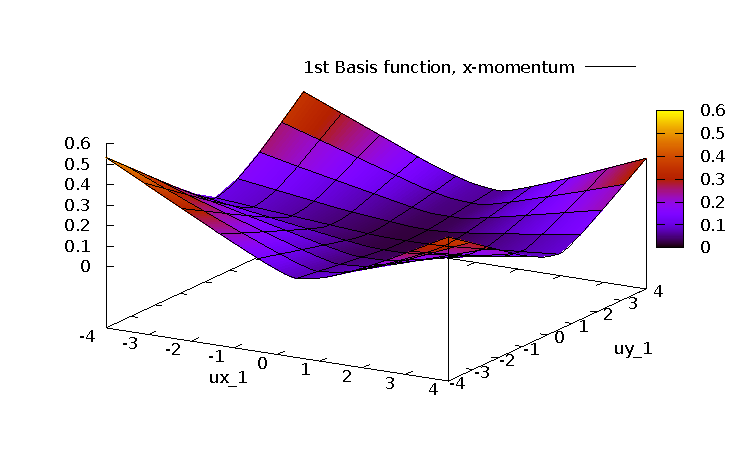
\includegraphics[scale=\zoomfactor]{{{ord1_varying_ux1_uy1_differing_ux2_uy2_1_1/10.0_10.0_10.0_x_1.0_0.0_y_1.0_0.0f00}}}
  }
  \subfigure[1st basis function, $y$-momentum -- 3rd basis function, $x$-momentum is the mirror image mirrored by the plane $u_{x,1}=u_{y,1}$.] {
    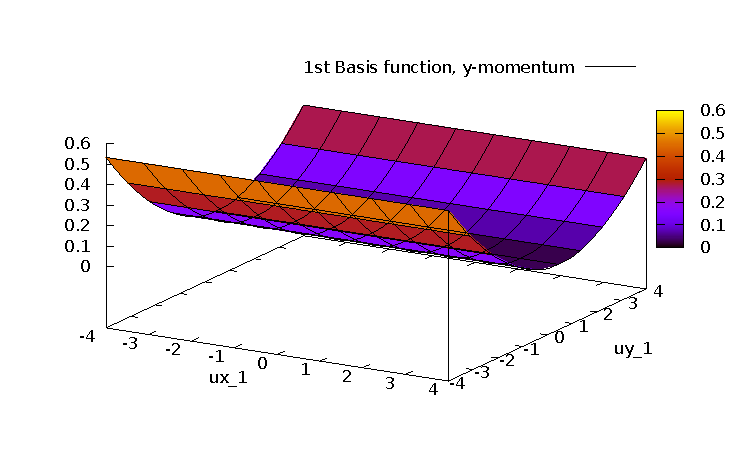
\includegraphics[scale=\zoomfactor]{{{ord1_varying_ux1_uy1_differing_ux2_uy2_1_1/10.0_10.0_10.0_x_1.0_0.0_y_1.0_0.0f01}}}
  }
  \subfigure[2nd basis function, $x$-momentum] {
    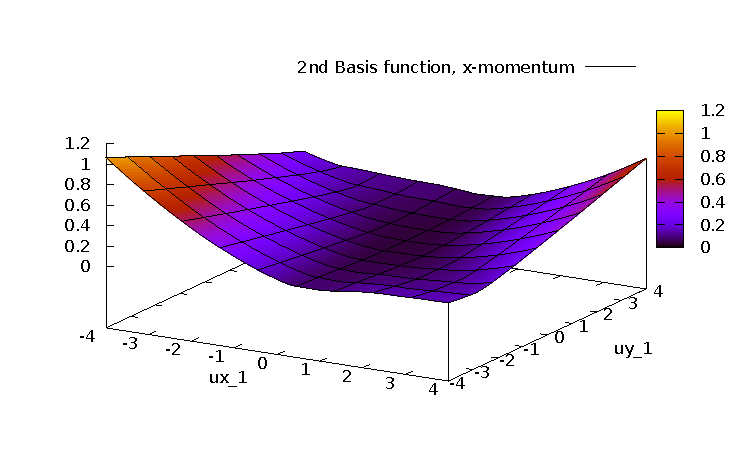
\includegraphics[scale=\zoomfactor]{{{ord1_varying_ux1_uy1_differing_ux2_uy2_1_1/10.0_10.0_10.0_x_1.0_0.0_y_1.0_0.0f02}}}
  }
  \subfigure[2nd basis function, $y$-momentum] {
    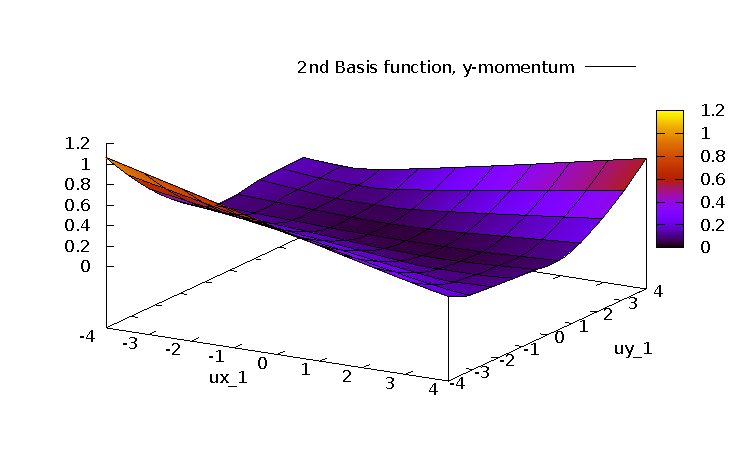
\includegraphics[scale=\zoomfactor]{{{ord1_varying_ux1_uy1_differing_ux2_uy2_1_1/10.0_10.0_10.0_x_1.0_0.0_y_1.0_0.0f03}}}
  }
  % \subfigure[] {
  %   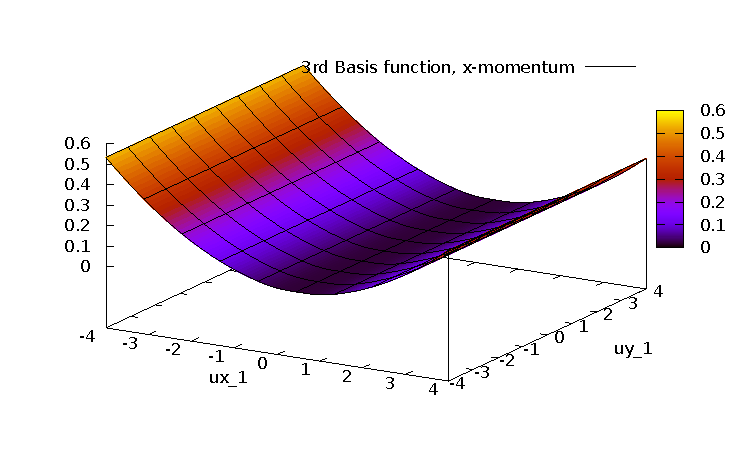
\includegraphics[scale=\zoomfactor]{{{ord1_varying_ux1_uy1_differing_ux2_uy2_1_1/10.0_10.0_10.0_x_1.0_0.0_y_1.0_0.0f04}}}
  % }
  % \subfigure[] {
  %   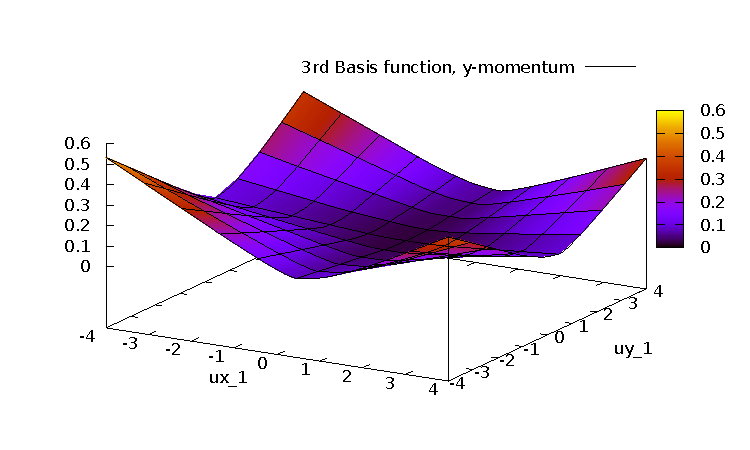
\includegraphics[scale=\zoomfactor]{{{ord1_varying_ux1_uy1_differing_ux2_uy2_1_1/10.0_10.0_10.0_x_1.0_0.0_y_1.0_0.0f05}}}
  % }
\caption{Error plots for varying $u_{x,1}$ and $u_{y,1}$. All heights are set to 10, all momentums to 0. Note that the $y$-momentum and $x$-momentum of the second basis functions are mirror images by the plane $u_{x,1}=u_{y,1}$. Similarily, e.g. the $x$-momentum of the first basis function is a mirror-image of the $y$-momentum of the third basis function.}
\label{fig:ord1_varying_ux1_uy1_differing_ux2_uy2_1_1}
\end{figure}

%%% Local Variables:
%%% TeX-master: "../results.tex"
%%% End:
